\documentclass{beamer}
\usepackage[english]{babel}
\usetheme{default}

\author{{\scriptsize T. Fossati, P. Giacomin, S. Loreto, M. Rossini}}
\title{CoAP Options for Sleepy Nodes}
\institute{{\large IETF 83, Paris}}
\date{}

\begin{document}

\begin{frame}[plain]
 \titlepage
\end{frame}

%%
%% Intro
%% 
\begin{frame}{Intro}

\begin{itemize}
 \item Two I-Ds for three Options :-)
 \item Extend Proxies capabilities to help Sleepy nodes participate in CoAP networks
 \item Each Option employs a different technique to solve specific (orthogonal) issues that surface when the \emph{always on} postulate is negated
\end{itemize}

\end{frame}

\begin{frame}{Options}

\begin{itemize}
 \item \textbf{Publish.}  Allow generic CoAP nodes to interact with a resource hosted at a sleepy node by (temporarily) delegating the resource to a Proxy;
 \vspace{.3cm}
 \item \textbf{Sleepy.}  Allow end to end communication between two sleepy nodes using the Proxy as a \emph{store and forward} agent;
 \vspace{.3cm}
 \item \textbf{Monitor.}  Make Observe bootstrap possible in case two sleepy nodes are involved.
\end{itemize}

\end{frame}


%%
%% Publish option 
%%
\begin{frame}{Publish \hspace{5cm} {\tiny \texttt{draft-fossati-core-publish-monitor-options-01}}}

\begin{itemize}
 \item Sleepy node asks Proxy to \emph{fully} serve its resource(s)
 \item Handle the whole delegation life-time: \mbox{\small{Publish $\rightarrow$ Update $\rightarrow$ ... $\rightarrow$ Update $\rightarrow$ (implicit) Remove}}
 \item Sleepy node may specify allowed methods %%(support writable resources, default GET only)
\end{itemize}

\end{frame}

%%
%% Publish (pic: disco)
%%
\begin{frame}{(0) Discover the supporting Proxy}
 \begin{center}
  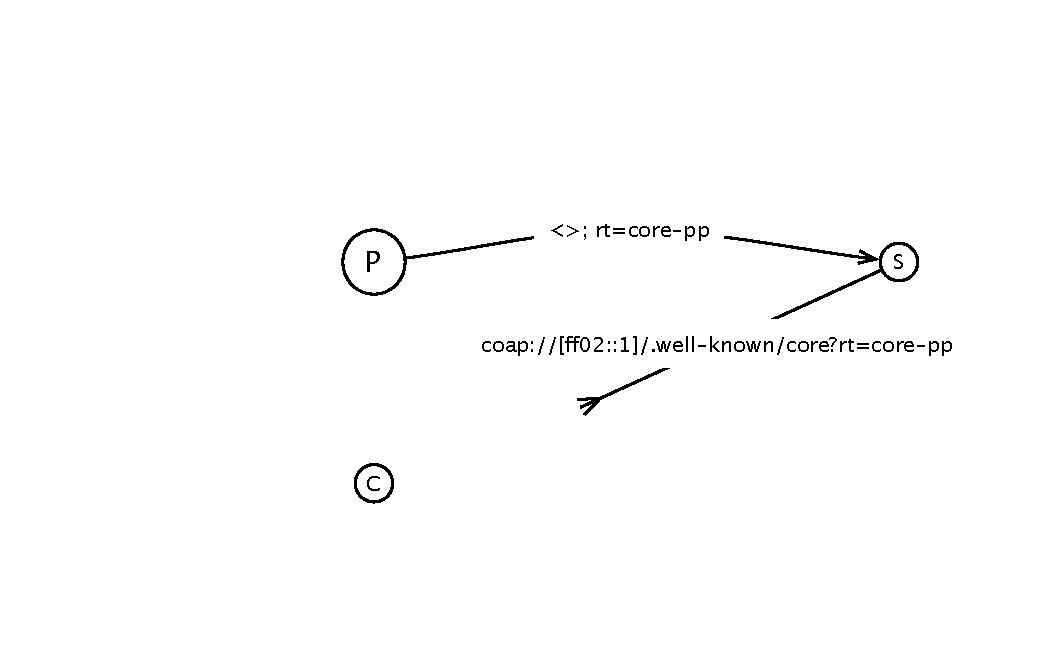
\includegraphics[width=\textwidth]{../../share/images/publish-1.pdf}
 \end{center}
\end{frame}


%%
%% Publish (pic: publish resource)
%%
\begin{frame}{(1) Publish resource}
 \begin{center}
  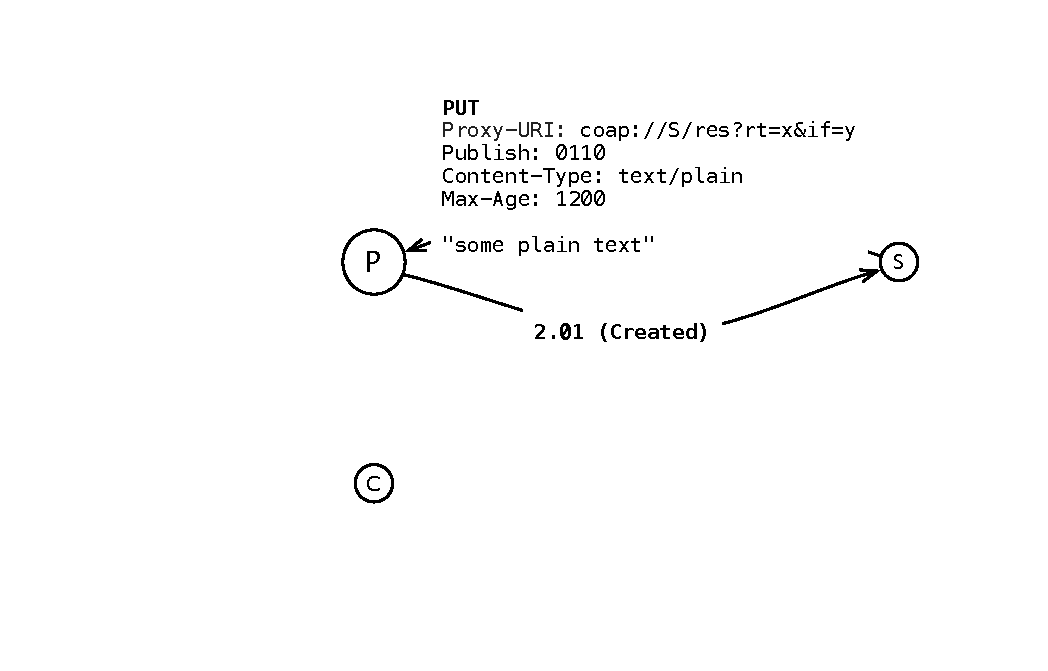
\includegraphics[width=\textwidth]{../../share/images/publish0.pdf}
 \end{center}
\end{frame}

%%
%% Publish (pic: discovery by 3rd parties)
%%
\begin{frame}{(1.5) Discovery by 3rd parties through Proxy}
 \begin{center}
  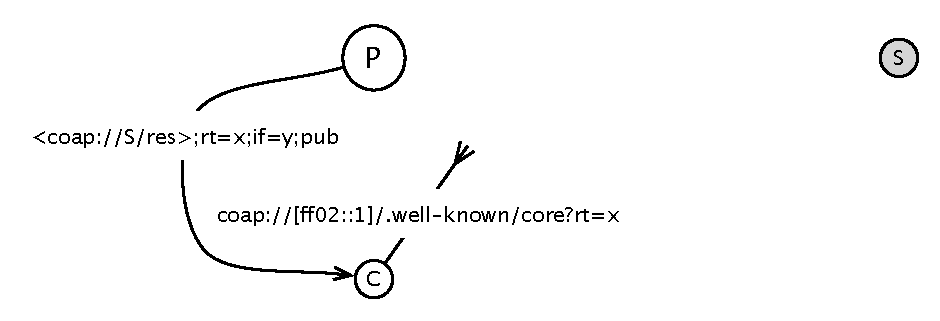
\includegraphics[width=\textwidth]{../../share/images/publish-disco.pdf}
 \end{center}
\end{frame}

%%
%% Publish (pic: retrieve published resource)
%%
\begin{frame}{(2) Act on published resource}
 \begin{center}
  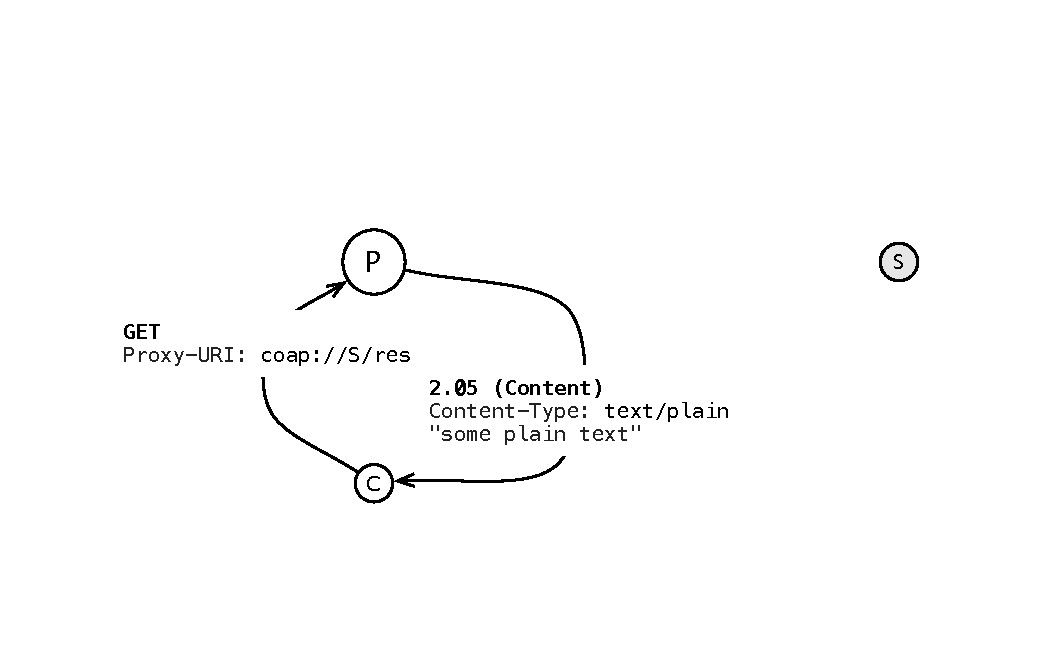
\includegraphics[width=\textwidth]{../../share/images/publish1.pdf}
 \end{center}
\end{frame}

%%
%% Publish (pic: update published resource)
%%
\begin{frame}{(3) Update published resource}
 \begin{center}
  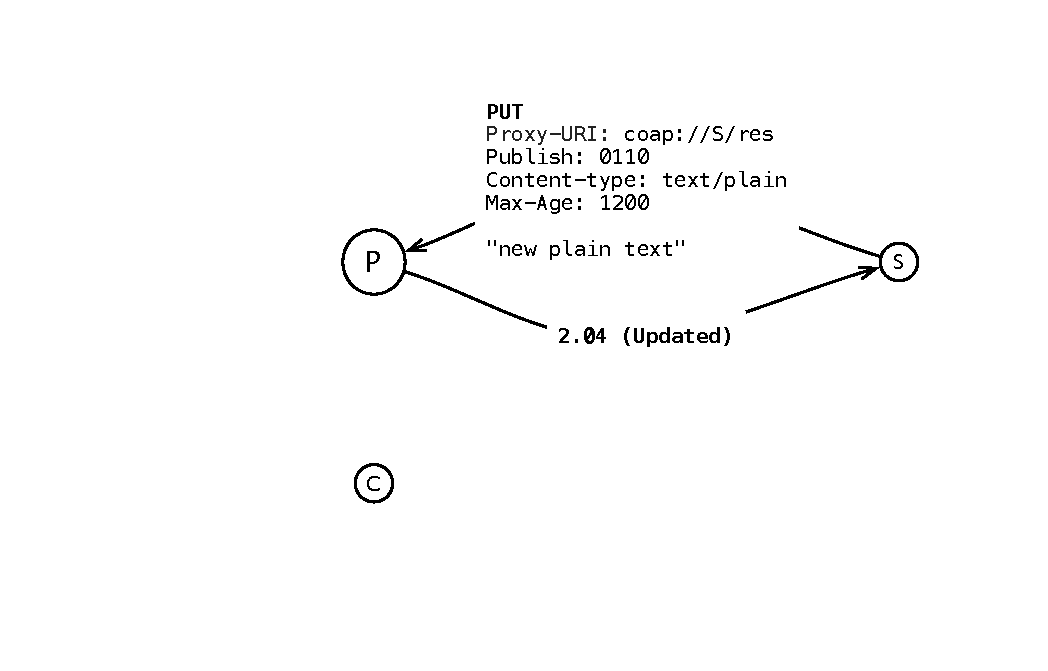
\includegraphics[width=\textwidth]{../../share/images/publish2.pdf}
 \end{center}
\end{frame}

%%
%% Publish (pic: retrieve published resource)
%%
\begin{frame}{(4) Act on updated resource}
 \begin{center}
  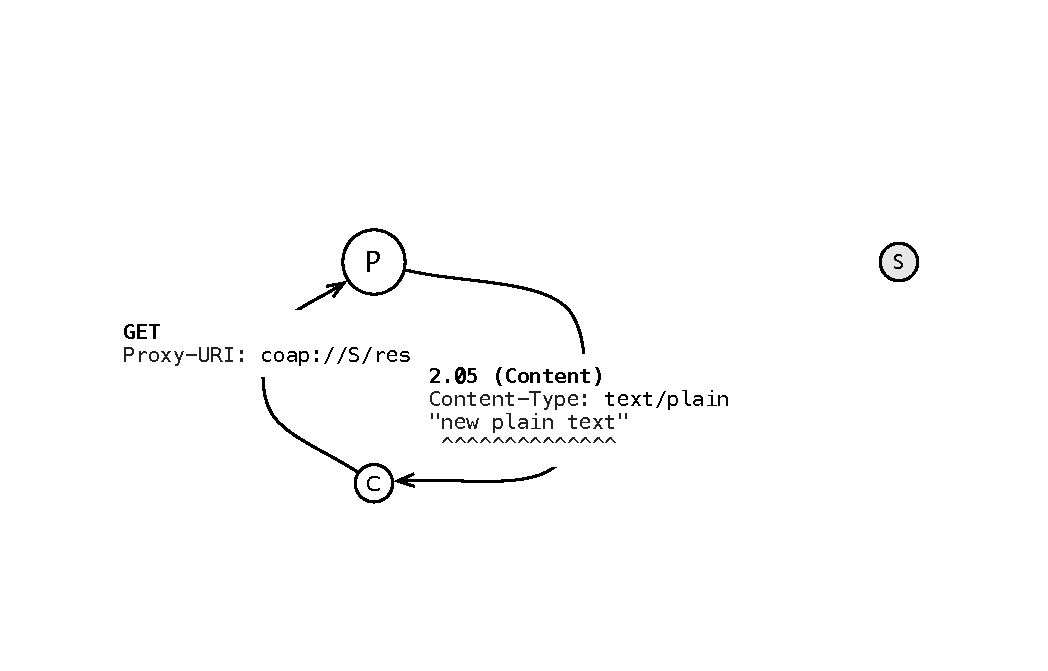
\includegraphics[width=\textwidth]{../../share/images/publish3.pdf}
 \end{center}
\end{frame}

%%
%% Publish (pic: remove delegation)
%%
\begin{frame}{(5) Remove delegation}
 \begin{center}
  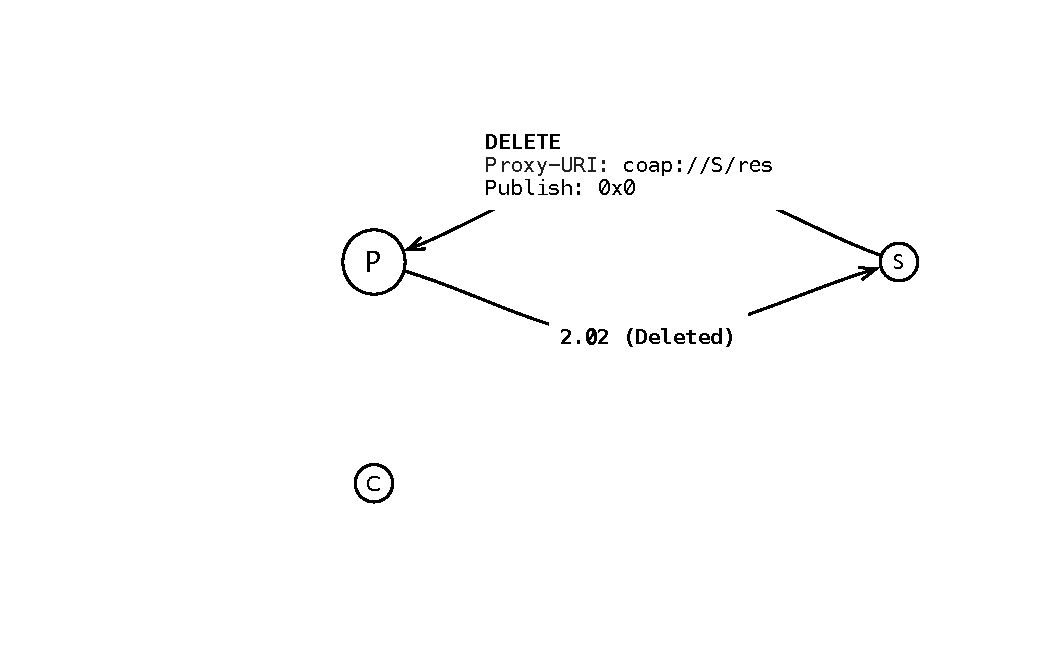
\includegraphics[width=\textwidth]{../../share/images/publish4.pdf}
 \end{center}
\end{frame}

%%
%% Publish (pic: removal)
%%
\begin{frame}{(6) Effect of delegation removal}
 \begin{center}
  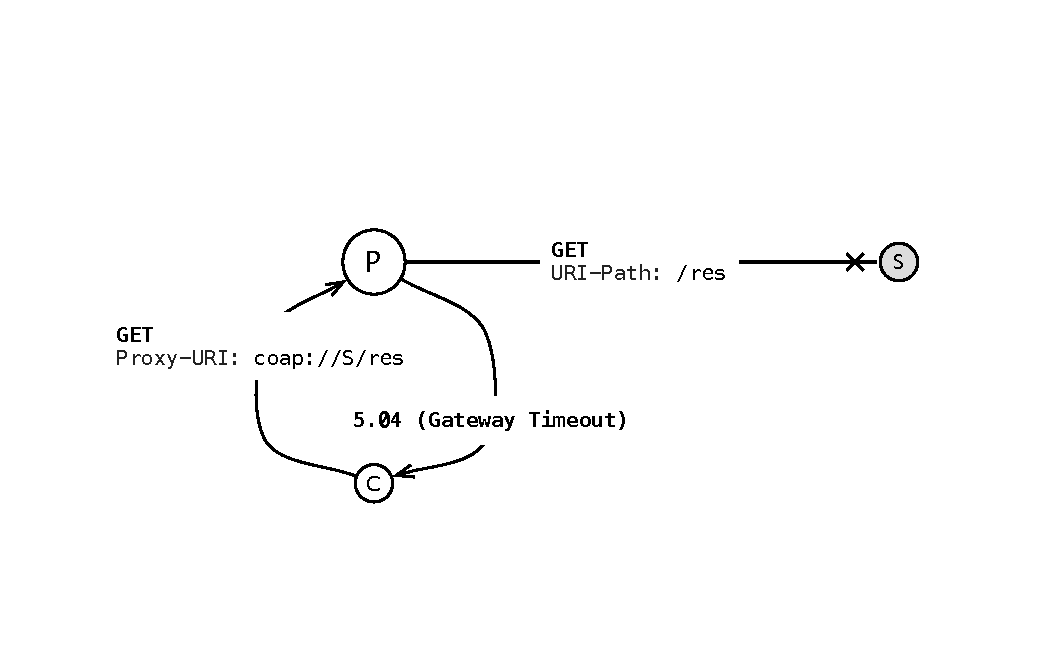
\includegraphics[width=\textwidth]{../../share/images/publish5.pdf}
 \end{center}
\end{frame}

%%
%% Pro
%%
\begin{frame}{The Good}

\begin{itemize}
 \item No URI proliferation %% the resource original URI is the only way to access the resource
 \item No state has to be maintained on sleepy client
 \item The sleepy node may never need to listen on the radio
 \item Explicit delegation lifetime
\end{itemize}
\end{frame}

\begin{frame}{The Good (cont)}
\begin{itemize}
 \item Support writable resources through methods' mask
 \item Support Observe
 \item Delegation of data and meta is \emph{atomic}
 \item Trivial patch to the Proxy logics 
\end{itemize}
\end{frame}

\begin{frame}[fragile]{The Good (cont)}


{\tiny 
\begin{verbatim}
$ git diff
@@ -249,6 +251,46 @@ ec_cbrc_t proxy_req(ec_server_t *srv, void *u0, struct timeval *u1, bool u2)
+    /* Catch Publish requests. */
+    if (m == EC_COAP_PUT && ec_request_get_publish(srv, &mask) == 0)
+    {
+        ec_mt_t mt;
+        size_t pload_sz;
+        uint32_t max_age;
+
+        if (ec_request_get_max_age(srv, &max_age))
+            max_age = 3600;
+
+        if (ec_request_get_content_type(srv, &mt))
+            mt = EC_MT_TEXT_PLAIN;
+
+        const uint8_t *pload = ec_request_get_payload(srv, &pload_sz);
+
+        dbg_err_if ((res = ec_resource_new(uri, mask, max_age)) == NULL);
+        dbg_err_if (ec_resource_add_rep(res, pload, pload_sz, mt, NULL));
+        dbg_err_if (ec_filesys_put_resource(g_ctx.cache, res));
+        res = NULL;
+
+        dbg_err_if (ec_register_cb(g_ctx.coap, uri, cache_serve, NULL));
+
+        dbg_if (ec_response_set_code(srv, EC_CREATED));
+        return EC_CBRC_READY;        
+    }
\end{verbatim}
}
\end{frame}

\begin{frame}{The Bad}
\begin{itemize}
 \item Can't go through Proxies (necessarily stops at first Proxy)
\end{itemize}
\end{frame}

%%
%% Open issues
%%
\begin{frame}{Open issues}

\begin{itemize}
 \item Need \emph{strong mutual authentication} to authorize the delegation (and subsequent ops -- i.e. updates and deletion) on the resource
 \item Need to be coerced to one only delegation relationship to ensure consistency
 \item How key material is supposed to be exported in case the published resource is \texttt{coaps} ?
\end{itemize}

\end{frame}


%%
%% Sleepy option 
%%
\begin{frame}{Sleepy  \hspace{6cm} {\tiny \texttt{draft-giacomin-core-sleepy-option-00}}}

\begin{itemize}
 \item Use Proxy as \emph{store and forward} agent for Sleepy to Sleepy messaging
 \item CON/NON $+$ Request/Response agnostic
 \item Sleepy nodes inform Proxy about their behavior
 \item Sleepy Option hits only the first Proxy encountered, so it works in any topology
 \item Sleepy Option doesn't need to be understood by both ends
 \item Sleepy node needs only to know his own Proxy
\end{itemize}

\end{frame}

\begin{frame}[fragile]{Information provided to Proxy}

\begin{description}
 \item[LEFT] \# of msec that the sending node is left before going off-duty.  Max value allows for 71582 minutes.
 \item[SLEEP] \# of msec that the sending node is off-duty.  Max value allows for 71582 minutes (i.e. approx. 50 days).
 \item[WAKE] \# of msec that the sending node is on-duty (optional).
\end{description}
\end{frame}

%%
%% Sleepy (1)
%%
\begin{frame}{Sleepy Seq Diagram (1)}
 \begin{center}
  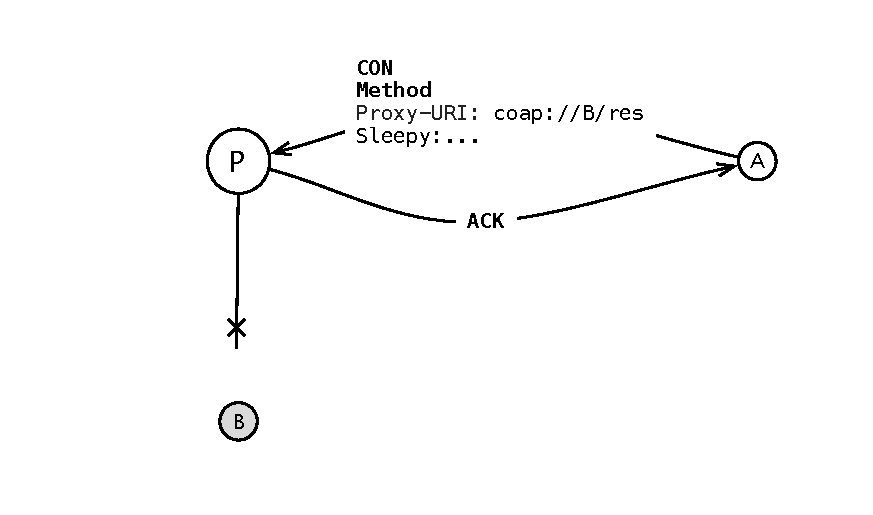
\includegraphics[width=\textwidth]{../../share/images/sleepy1.pdf}
 \end{center}
\end{frame}

%%
%% Sleepy (2)
%%
\begin{frame}{Sleepy Seq Diagram (2)}
 \begin{center}
  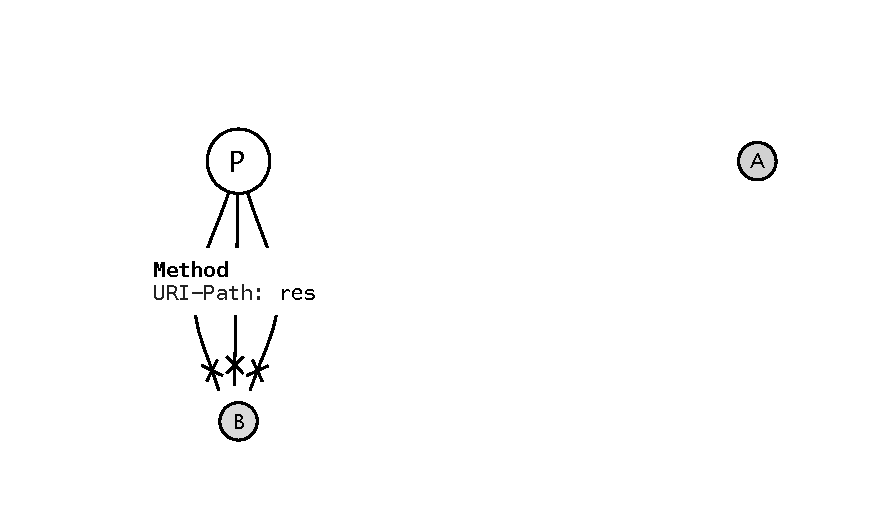
\includegraphics[width=\textwidth]{../../share/images/sleepy2.pdf}
 \end{center}
\end{frame}

%%
%% Sleepy (3)
%%
\begin{frame}{Sleepy Seq Diagram (3)}
 \begin{center}
  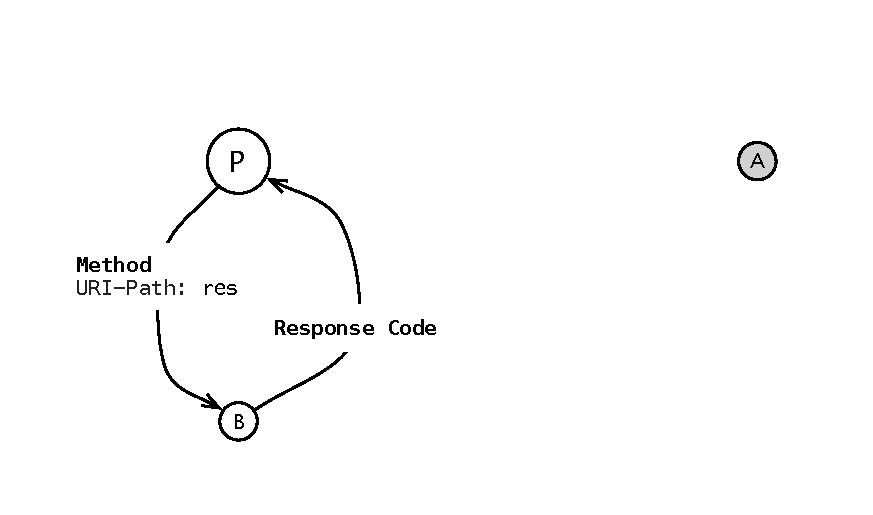
\includegraphics[width=\textwidth]{../../share/images/sleepy3.pdf}
 \end{center}
\end{frame}

%%
%% Sleepy (4)
%%
\begin{frame}{Sleepy Seq Diagram (4)}
 \begin{center}
  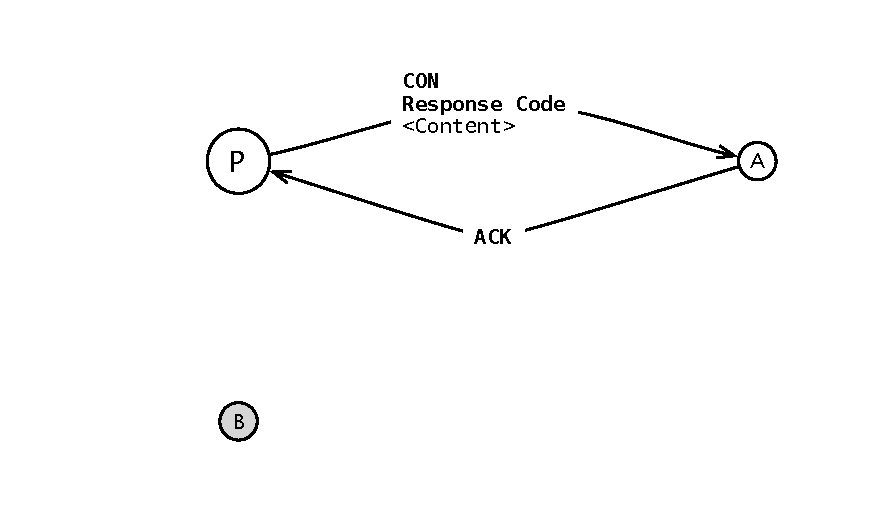
\includegraphics[width=\textwidth]{../../share/images/sleepy4.pdf}
 \end{center}
\end{frame}

\begin{frame}{Sleepy partitioning amendment and open issues}

\begin{itemize}
 \item Encode in Seconds (finer granularity is a matter of RDC)
 \item Open Issue: Reduce to LEFT, SLEEP and WAKE to 24 bits (approx 166 days) vs 32 bits (approx 136 years), keep SLEEP on 32 bits?
\end{itemize}


\end{frame}

%%
%% Monitor option 
%%
\begin{frame}{Monitor \hspace{5cm} {\tiny \texttt{draft-fossati-core-publish-monitor-options-01}}}

\begin{itemize}
 \item Allow Observe to work in presence of Sleepy nodes %% bootstrap + lost notifications
 \item Solve bootstrap issue in case {\scriptsize $wake(S_1) \cap wake(S_2) = \emptyset$}
\end{itemize}

\end{frame}


%%
%% Monitor (pic: create monitor)
%%
\begin{frame}{(1) Create the Monitor resource}
 \begin{center}
  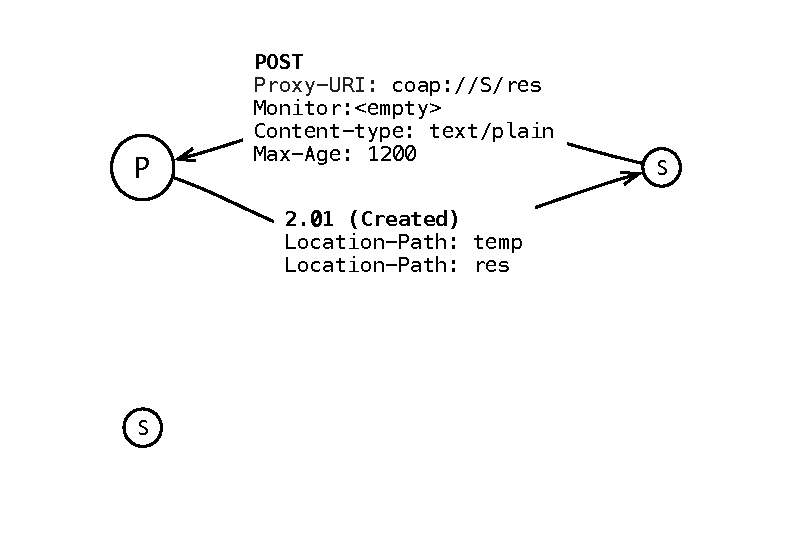
\includegraphics[width=\textwidth]{../../share/images/monitor1.pdf}
 \end{center}
\end{frame}

%%
%% Monitor (pic: observe in action)
%%
\begin{frame}{(2) Proxy updates the Monitor}
 \begin{center}
  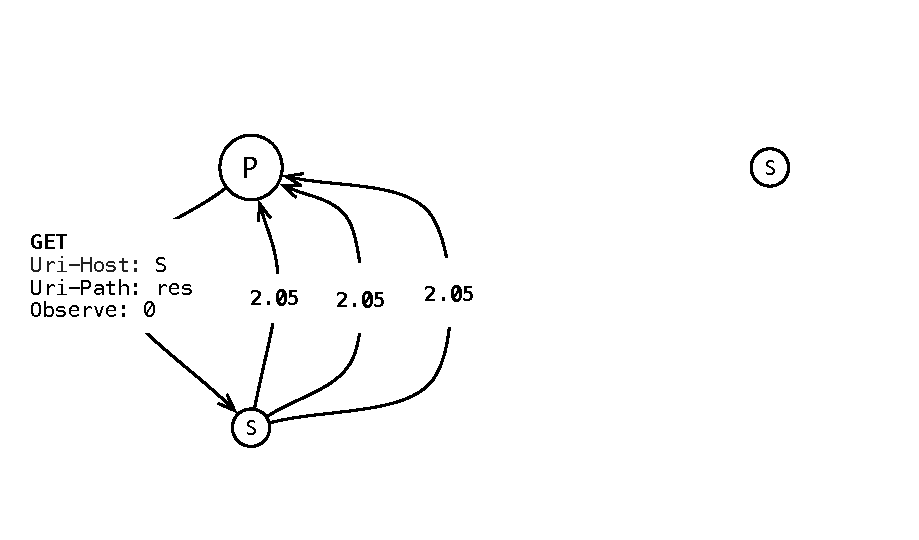
\includegraphics[width=\textwidth]{../../share/images/monitor2.pdf}
 \end{center}
\end{frame}

%%
%% Monitor (pic: Wake up and get last value)
%%
\begin{frame}{(3) Wake up and get the Monitor value}
 \begin{center}
  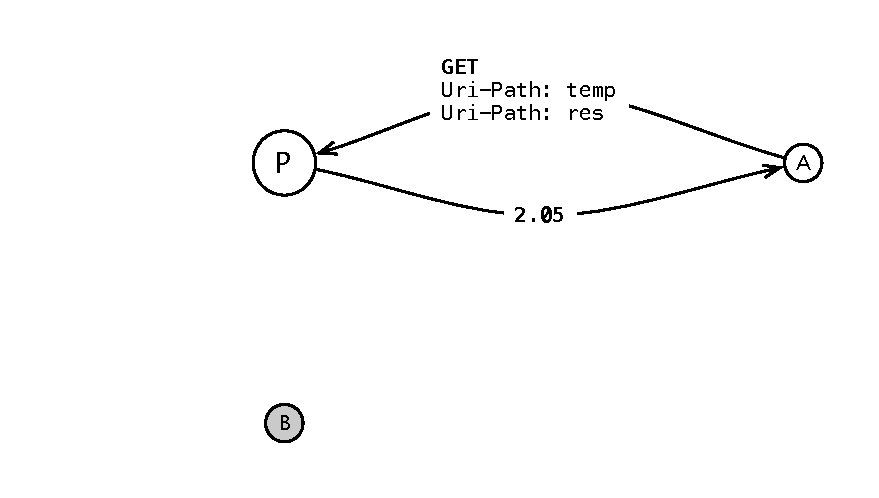
\includegraphics[width=\textwidth]{../../share/images/monitor3.pdf}
 \end{center}
\end{frame}



\end{document}
